\chapter{Hasil dan Pembahasan}

\section{Analisis pada Sistem Operasi Linux Sungguhan}

Dengan bantuan perangkat lunak virtualisasi UTM, analisis sistem penanganan notifikasi dan sisten kontrol media pada sistem operasi Linux sungguhan dilakukan pada sebuah \textit{virtual machine} (bertindak sebagai komputer referensi) yang menjalankan sistem operasi Ubuntu 22.04 (LTS) edisi arsitektur ARM 64-bit dan berjalan di atas perangkat komputer \textit{host} MacBook Air keluaran tahun 2020 (berprosesor M1) bersistem operasi macOS 13 "Ventura".

\begin{figure}[h]
    \centering
    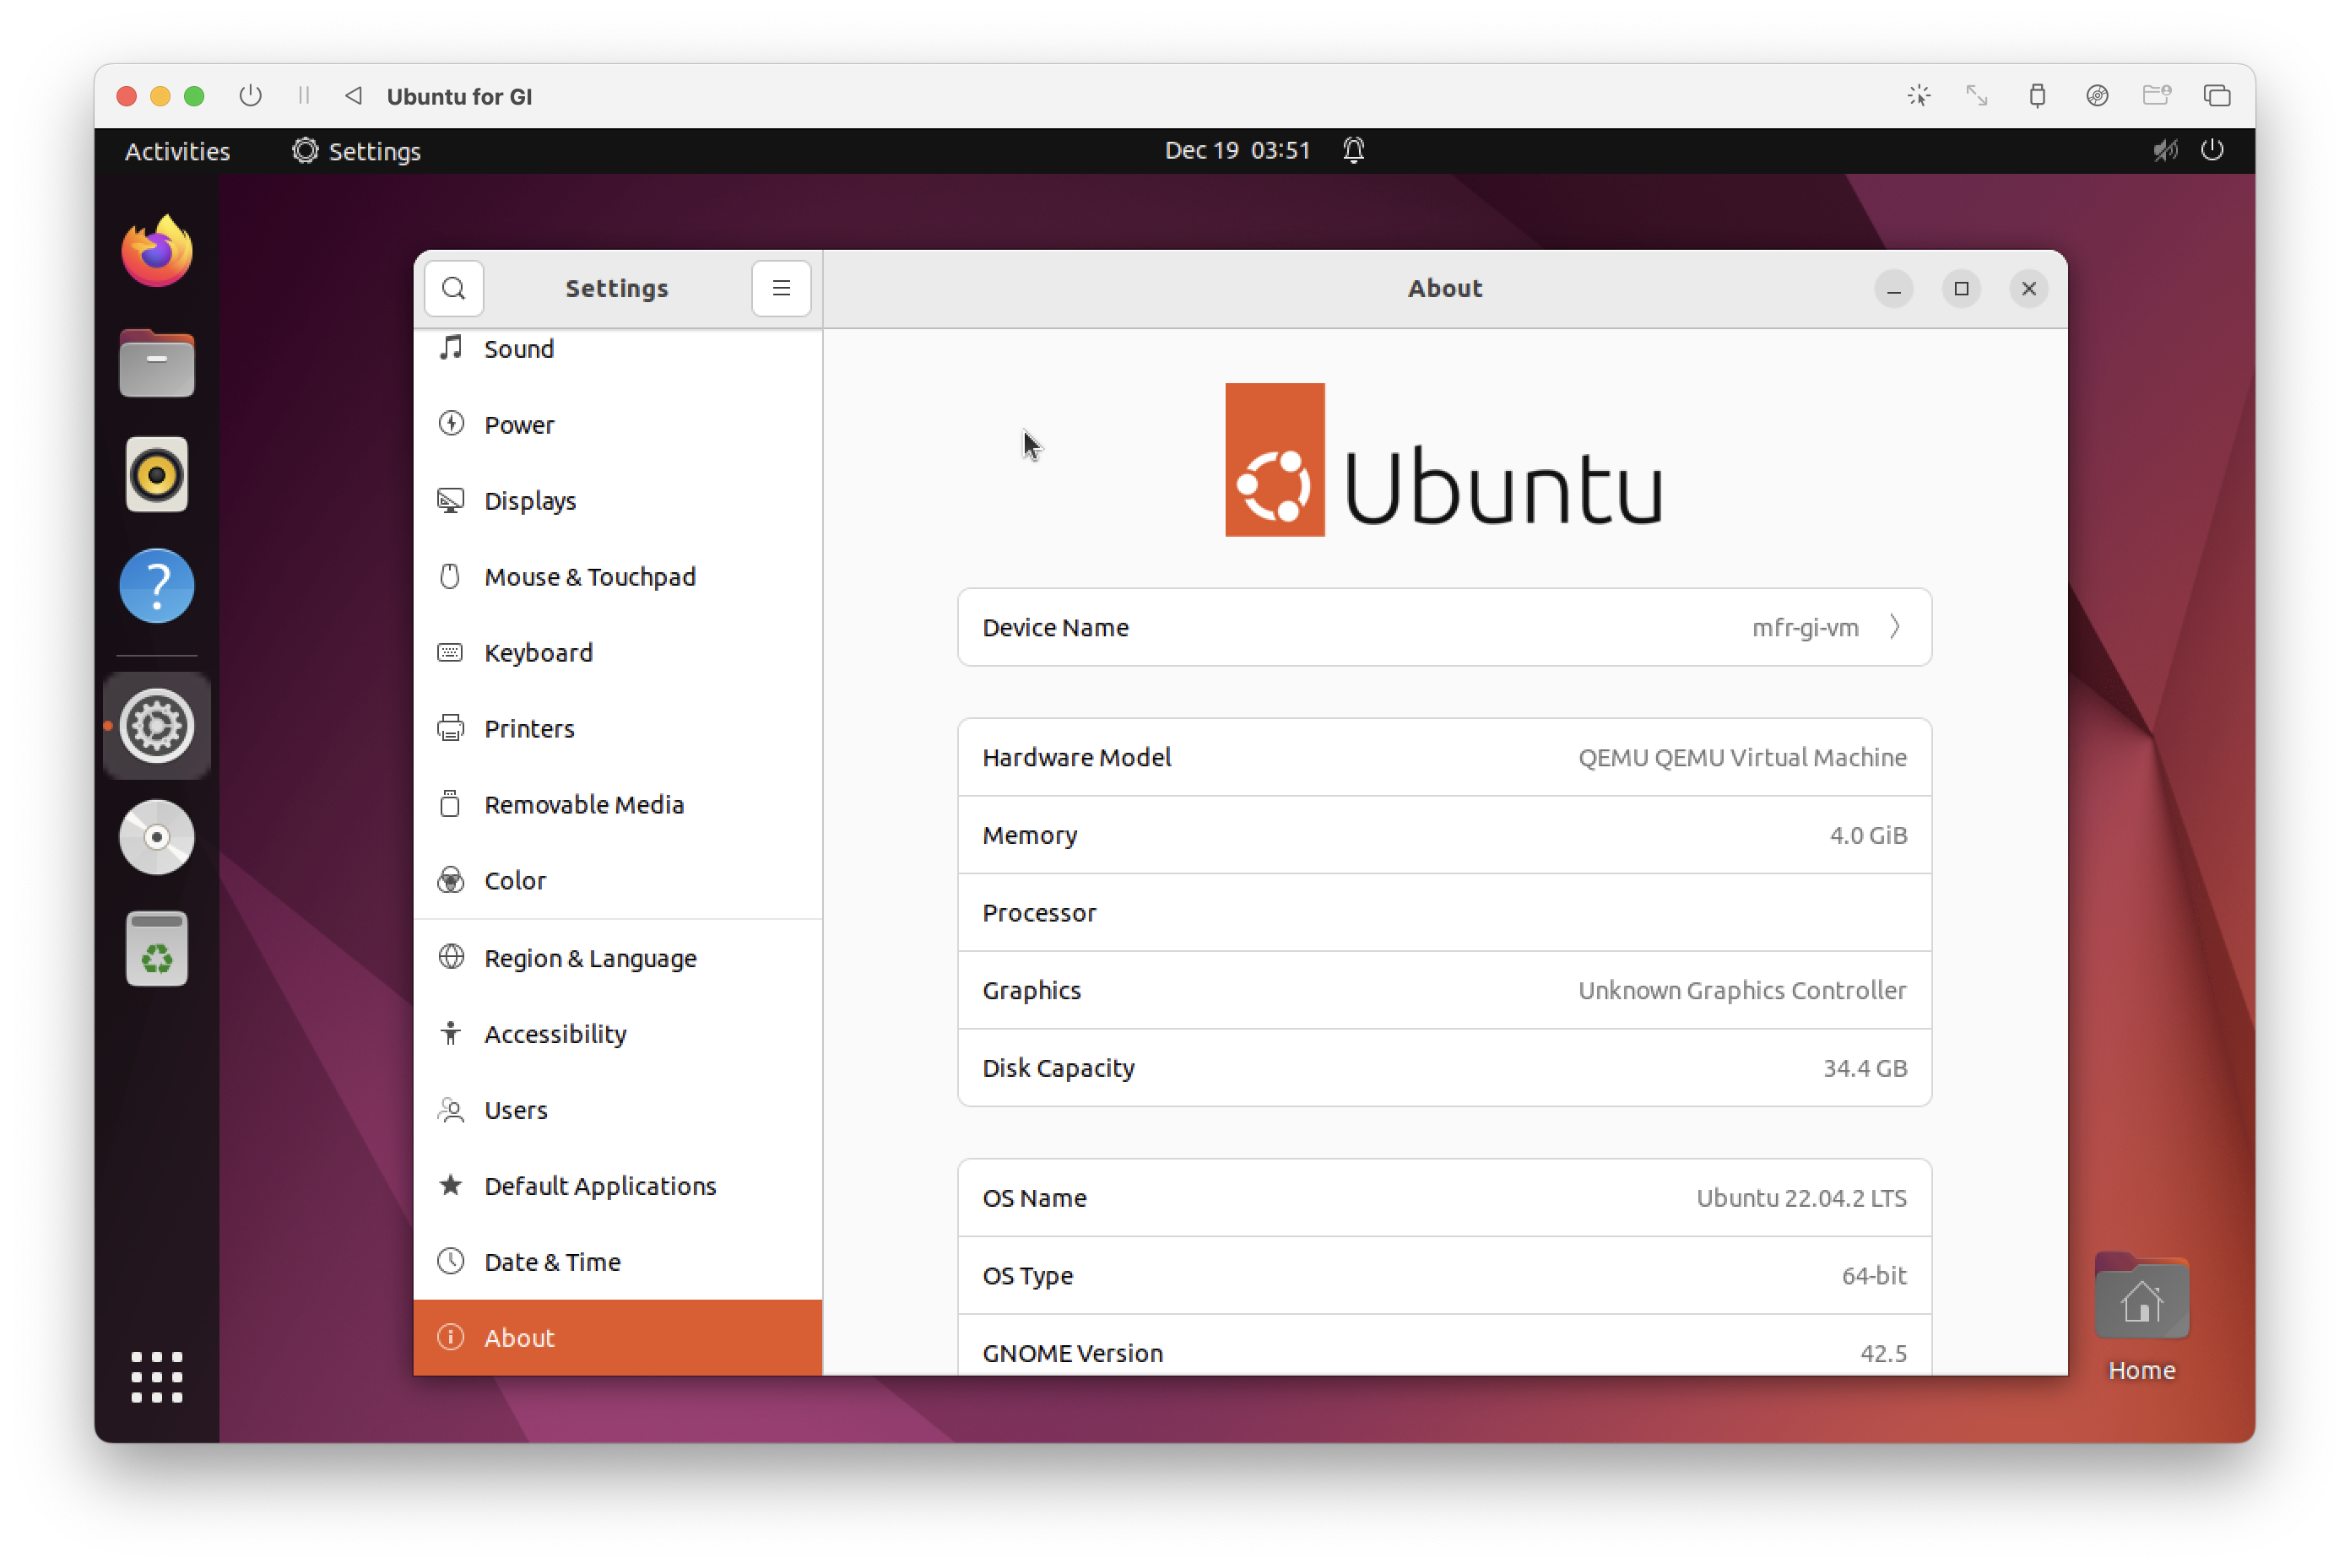
\includegraphics[width=0.75\linewidth]{archives//contents-template-pak-prapto//chapter-4/Screenshot 2023-12-19 at 10.51.04.png}
    \caption{Tangkapan layar \textit{virtual machine} Ubuntu 22.04 (LTS) yang sedang berjalan}
    \label{fig:enter-label}
\end{figure}

\subsection{Analisis Sistem Penanganan Notifikasi}

Pengelolaan sistem penanganan notifikasi pada sistem operasi Linux bergantung pada distribusi dan/atau lingkungan desktop (\textit{desktop environment}) yang digunakan, tetapi hampir seluruh implementasi penanganan notifikasi pada sistem operasi Linux berkomunikasi melalui bus perpesanan D-Bus. Uji coba sistem notifikasi pada Linux dapat dilakukan melalui berbagai cara, seperti
\begin{itemize}
    \item menggunakan perangkat lunak yang normalnya mengirimkan notifikasi (aplikasi \textit{e-mail}, aplikasi perpesanan, dan lain-lain),
    \item mensimulasikan pemanggilan metode (\textit{method}) objek D-Bus khusus yang bertugas menangani notifikasi dengan menggunakan alat (\textit{tool}) pengujian \verb|dbus-send| yang disediakan oleh paket perangkat lunak D-Bus itu sendiri, dan
    \item menggunakan alat (\textit{tool}) \verb|notify-send| yang memiliki fungsi tunggal mengirimkan notifikasi pada \textit{desktop} Linux.
\end{itemize}

Karena kepraktisannya, digunakan alat (\textit{tool}) \verb|notify-send| dalam pengujian awal ini. Alat \verb|notify-send| tersedia secara bawaan pada banyak distribusi Linux seperti Ubuntu dan Fedora. Mengutip halaman manual alat 

\subsection{Analisis Sistem Kontrol Media}

\section{Analisis Ekosistem pada Masing-Masing Platform (Linux dan Windows)}

\subsection{Analisis Sistem Penanganan Notifikasi}

\subsection{Analisis Sistem Kontrol Media}

\section{Pengembangan Perangkat Lunak FancyWSL}

\section{Perbandingan Hasil Penelitian dengan Hasil Terdahulu}
